\documentclass[12pt, a4paper, oneside]{ctexbook}
\usepackage{amsmath, amsthm, amssymb, hyperref, mathrsfs}
% 引入超链接hyperref
\usepackage{bm}% 加粗公式内字体bm
\usepackage{graphicx} %插入图片的宏包
\usepackage{float} %设置图片浮动位置的宏包
\usepackage{subfigure} %插入多图时用子图显示的宏包

\graphicspath{{../images/}}


% 超链接样式
\hypersetup{hidelinks,colorlinks=true,allcolors=black,pdfstartview=Fit,breaklinks=true}

% 标题,作者,时间
\title{{\Huge{\textbf{工程数学基础}}}}
% \href{超链接地址}{文本}引入超链接
\author{\href{https://space.bilibili.com/230105574}{DR\_CAN}}
\date{\today}



% 定理,定义,引理,推论,命题,例
\linespread{1.5}
\newtheorem{theorem}{定理}[section]
\newtheorem{definition}[theorem]{定义}
\newtheorem{lemma}[theorem]{引理}
\newtheorem{corollary}[theorem]{推论}
\newtheorem{example}[theorem]{例}
\newtheorem{proposition}[theorem]{命题}



% ------------------------------------------------------------------------------
% 文章主体
\begin{document}
% 编译标题
\maketitle
% ------------------------------------------------------------------------------



% 章节目录
\newpage
\pagenumbering{Roman}
\setcounter{page}{1}
\tableofcontents
\newpage
\setcounter{page}{1}
\pagenumbering{arabic}


% 正文
% 章节
\chapter{特征值与特征向量}

% \bm{}加粗公式内文本
在数学中,特别是线性代数中,对于一个给定的线性变换$\bm{A}$,它的特征向量$\bm{v}$经过这个线性变换的作用之后,得到的新向量仍然与原来的$\bm{v}$保持在同一条直线上,但其长度或方向也许会改变,即

$$ \bm{Av}=\bm {\lambda v} $$


其中$\bm{\lambda}$为标量,即特征向量的长度在该线性变换下缩放的比例,称为其特征值


%-----------------------------------------------------------------------------
% 小节
\section{线性变化}

 现有二维线性变化矩阵

$$
\bm{A}=
 \left[
    \begin{matrix}
        1 & 1 \\
        4 & -2 \\
    \end{matrix}
 \right]
 $$

以及一个向量

$$\bm{v_1}=
\left[
    \begin{matrix}
        1 \\ 2 \\
    \end{matrix}
\right]
$$

向量$\bm{v_1}$通过$\bm{A}$的线性变换,即

$$
\bm{A v_1}=
\left[
    \begin{matrix}
        1 & 1 \\
        4 & -2 \\
    \end{matrix}
\right]
\left[
    \begin{matrix}
        1 \\ 2 \\
    \end{matrix}
\right]=
\left[
    \begin{matrix}
        1 \times 1 + 1 \times 2 \\
        4 \times 1 + (-2) \times 2 \\
    \end{matrix}
\right]=
\left[
    \begin{matrix}
        3 \\ 0 \\
    \end{matrix}
\right]
$$


笛卡尔坐标系下$v_1$向量的$A$变化如图\ref{md230213001}所示


\begin{figure}[H] 
    %H为当前位置,!htb为忽略美学标准,htbp为浮动图形
    \centering %图片居中
    % width=0.80\texwidth表示图片占页面的80%宽度
    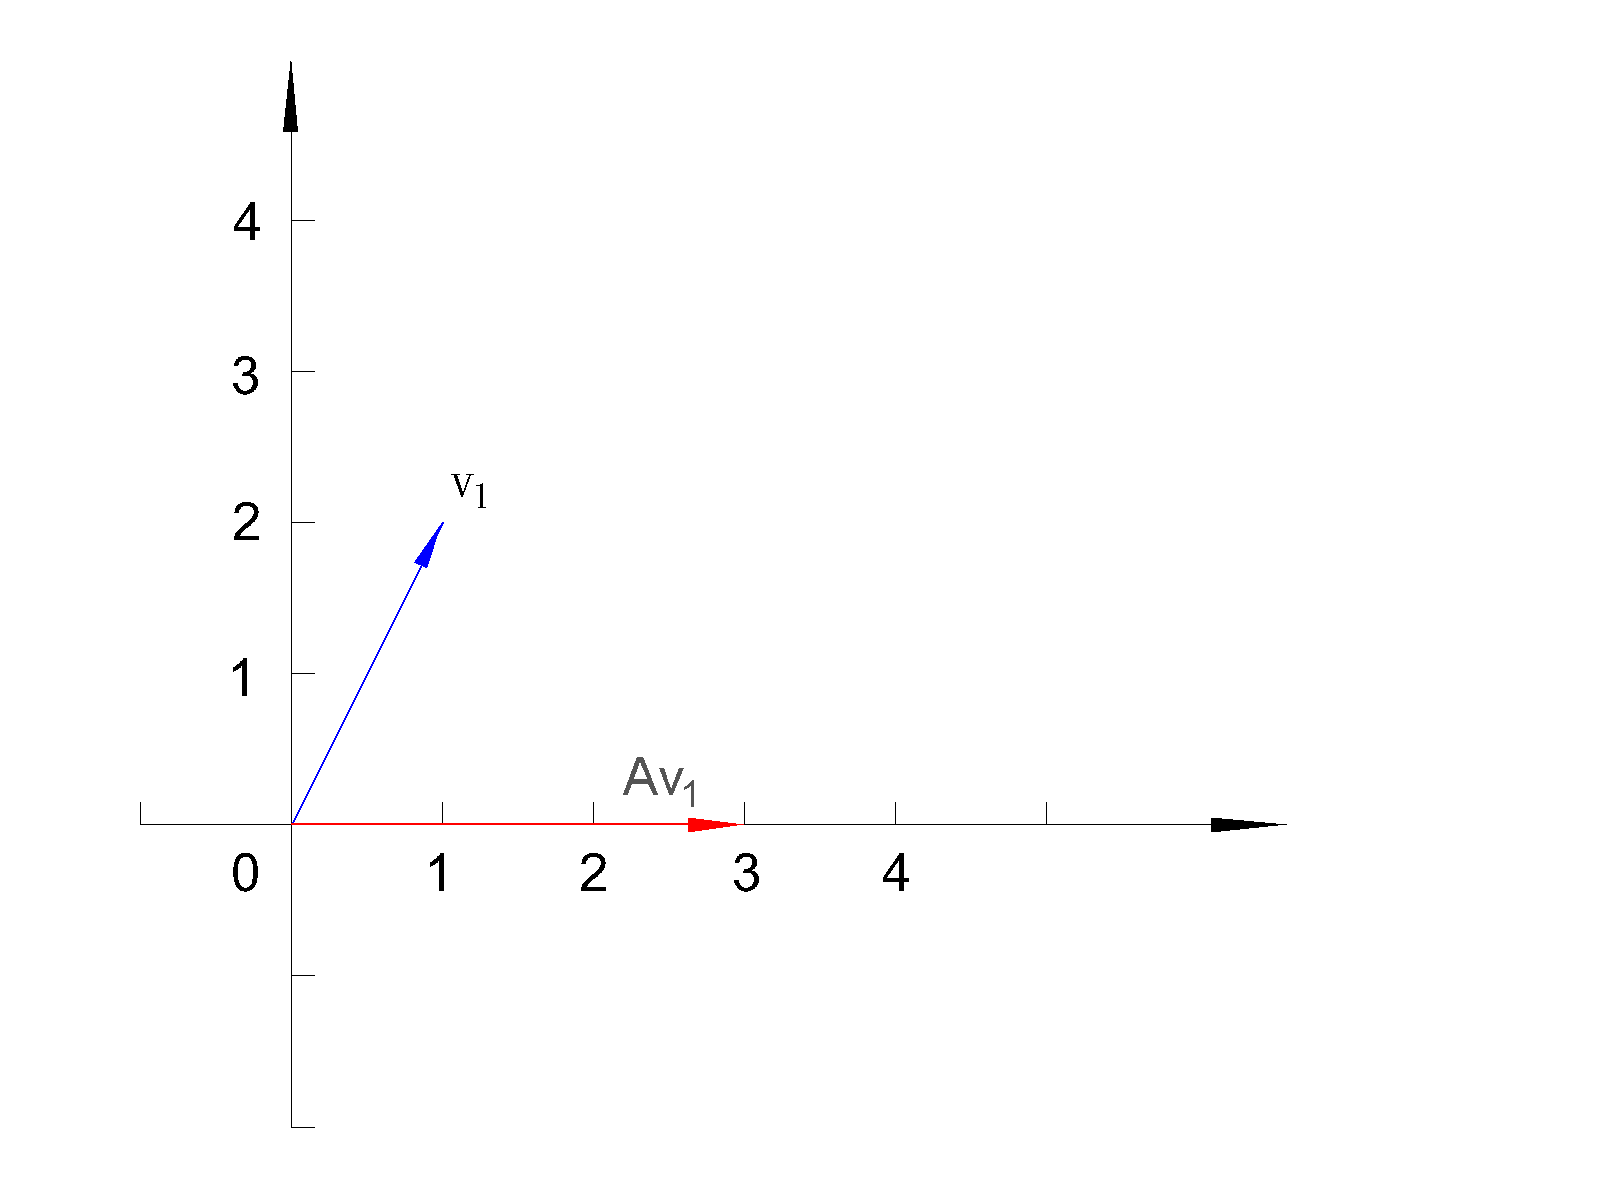
\includegraphics[width=0.80\textwidth]{md230213001.png}
    \caption{$v_1$向量的$A$变化} %图片标题
    \label{md230213001} %图片引用的标签
    % \label引用标签
\end{figure}

通过图\ref{md230213001}可以看出$v_1$通过$A$的线性变化后大小和方向都发生了变化

现有另一个向量

$$
v_2=
\left[
    \begin{matrix}
        1 \\ 1 \\
    \end{matrix}
\right]
$$

同样的对$v_2$进行$A$线性变化得到

$$
Av_2=
\left[
    \begin{matrix}
        1 & 1 \\
        4 & -2 \\
    \end{matrix}
\right]
\left[
    \begin{matrix}
        1 \\ 1 \\
    \end{matrix}
\right]=
\left[
    \begin{matrix}
        1 \times 1 + 1 \times 1 \\
        4 \times 1 + (-2) \times 1 \\
    \end{matrix}
\right]=
\left[
    \begin{matrix}
        2 \\ 2 \\
    \end{matrix}
\right]=
2\left[
    \begin{matrix}
        1 \\ 1 \\
    \end{matrix}
\right]=
2v_2
$$

$Av_2$与$v_2$在一条直线上,根据定义可知$v_2$是矩阵$A$的特征向量,缩放比例2即是特征值$\lambda$

\begin{figure}[H]
    \centering
    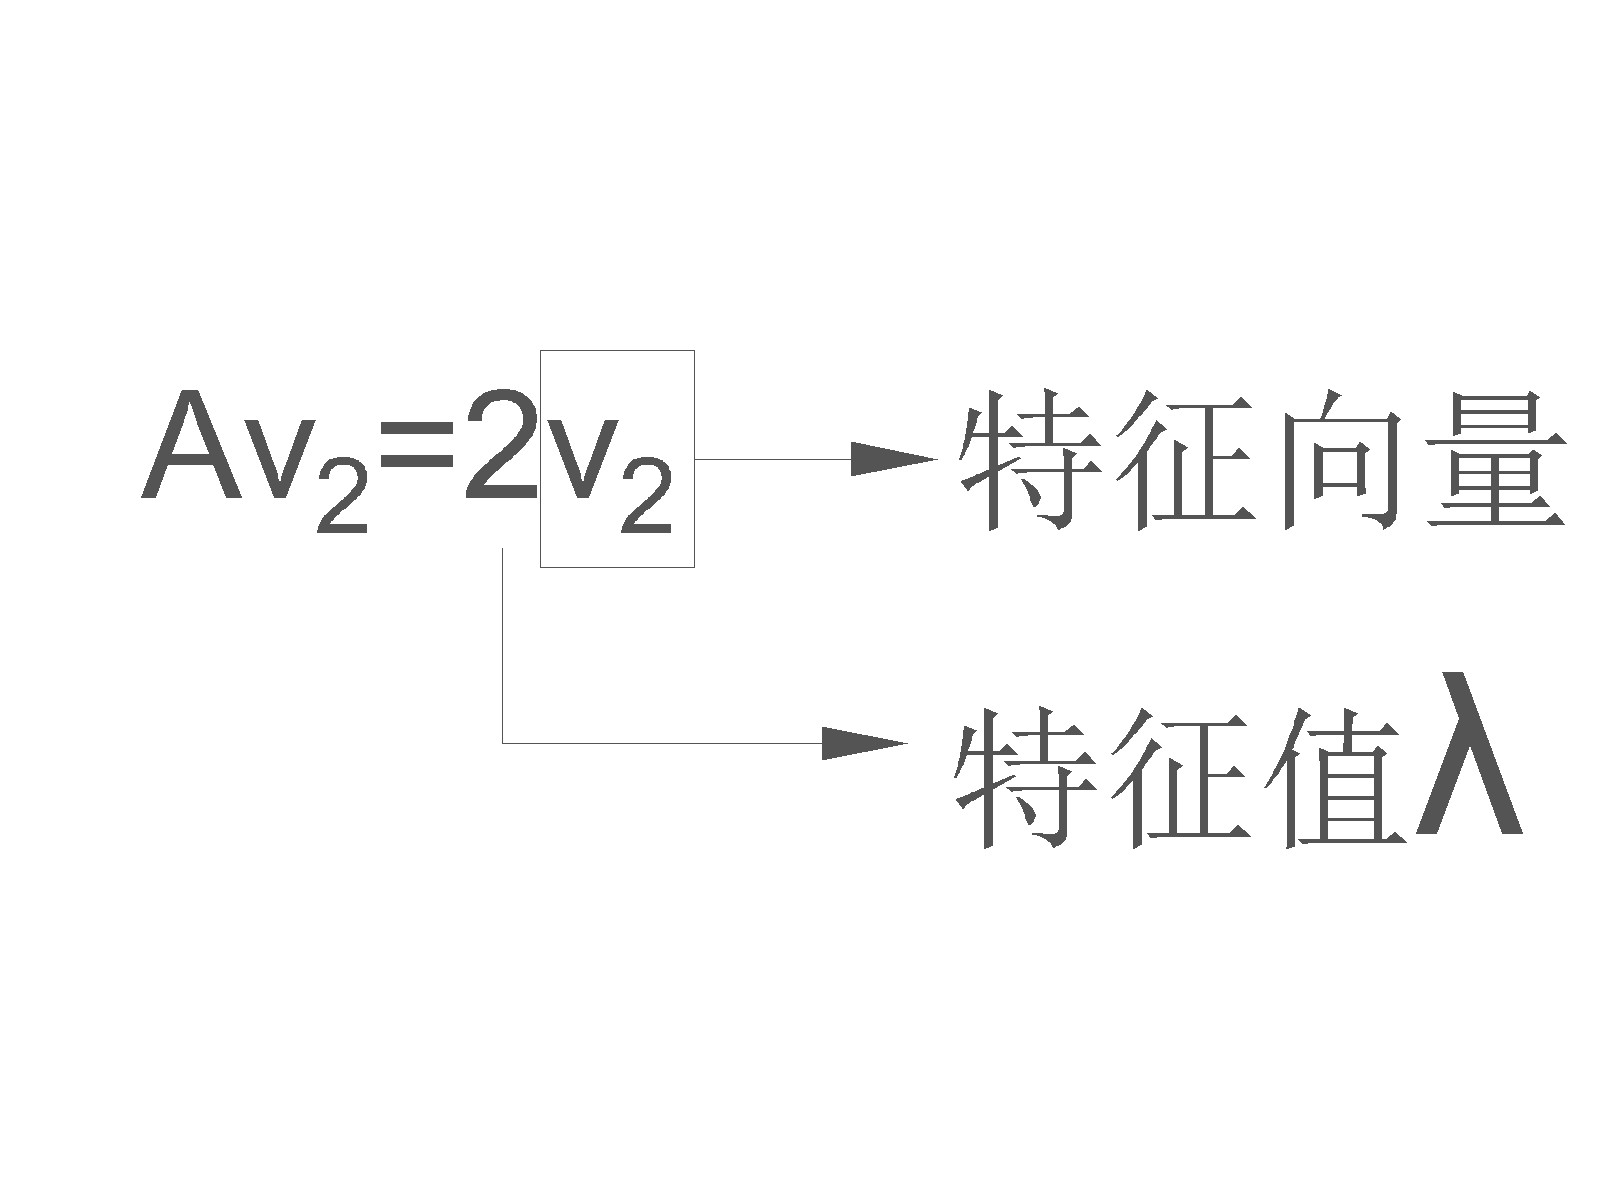
\includegraphics[width=0.3\textwidth]{md230215001.png}
    \label{md230215001}
\end{figure}

------------------------------------------------------------------------------
% 小节
\section{求解特征值特征向量}

求解矩阵的特征值和特征向量推导:
\begin{equation}
    Av=\lambda v
\end{equation}
\begin{equation} 
    Av-\lambda v=0
\end{equation}
\begin{equation}\label{eq1}
    (A-\lambda I)v=0
\end{equation}

此处$I$是一个单位矩阵

若式\ref{eq1}有非零解则有

$$
\begin{vmatrix}
    A-\lambda I
\end{vmatrix}
=0
$$

通过上式即可求得特征值$\lambda$,然后再将特征值带回式\ref{eq1}中即可得到特征向量。


\begin{example}
    现有矩阵
    $A=
    \left[
        \begin{matrix}
            1 & 1 \\
            4 & -2 \\
        \end{matrix}
    \right]
    $
    ,求其特征值和特征向量。




    解:
    $$
    A-\lambda I=
    \left[
        \begin{matrix}
            1 & 1 \\
            4 & -2 \\
        \end{matrix}
    \right]-
    \left[
        \begin{matrix}
            \lambda & 0 \\
            0 & \lambda \\
        \end{matrix}
    \right]=
    \left[
        \begin{matrix}
            1-\lambda & 1 \\
            4 & -2-\lambda \\
        \end{matrix}
    \right]
    $$


    \begin{align}
        \begin{vmatrix}
            A-\lambda I
        \end{vmatrix}=0
        \Rightarrow
        % \Rightarrow右向箭头
        \begin{vmatrix}
            1-\lambda & 1 \\
            4 & -2-\lambda \\
        \end{vmatrix}
        &=0
        \nonumber
        % \nonumber去掉编号
        \\
        (1-\lambda)(-2-\lambda)-1\times 4&=0
        \nonumber
        \\
        \lambda^2 + \lambda -6&=0
        \nonumber
        \\
        (\lambda-2)(\lambda+3)&=0
        \nonumber
    \end{align}
    $$
    \lambda_1=2,\lambda_2=-3
    $$

    此处$\lambda_1,\lambda_2$即是矩阵$A$的特征值

    \textcircled{1} 当$\lambda_1=-2$时,带入$(A-\lambda I=0)$,求解矩阵$A$的特征向量
    % \textcircled{}序号
    $$
    \left[
        \begin{matrix}
            1-2 & 1 \\
            4 & -2-2 \\
        \end{matrix}
    \right]
    v_1=0
    $$

    此处向量$v_1$即是特征值$\lambda_1$所对应的“$A$的特征向量”。

    $$
    \left[
        \begin{matrix}
            -1 & 1 \\
            4 & -4 \\
        \end{matrix}
    \right]
    \left[
        \begin{matrix}
            v_{11} \\
            v_{12} \\
        \end{matrix}
    \right]=0
    $$

    $$
    \begin{cases}
        -v_{11}+v_{12}=0 \\
        4v_{11}-4v_{12}=0 \\
    \end{cases}
    % cases括弧内公式
    \Rightarrow v_{11}=v_{12}
    $$

    \begin{figure}[H]
        \centering
        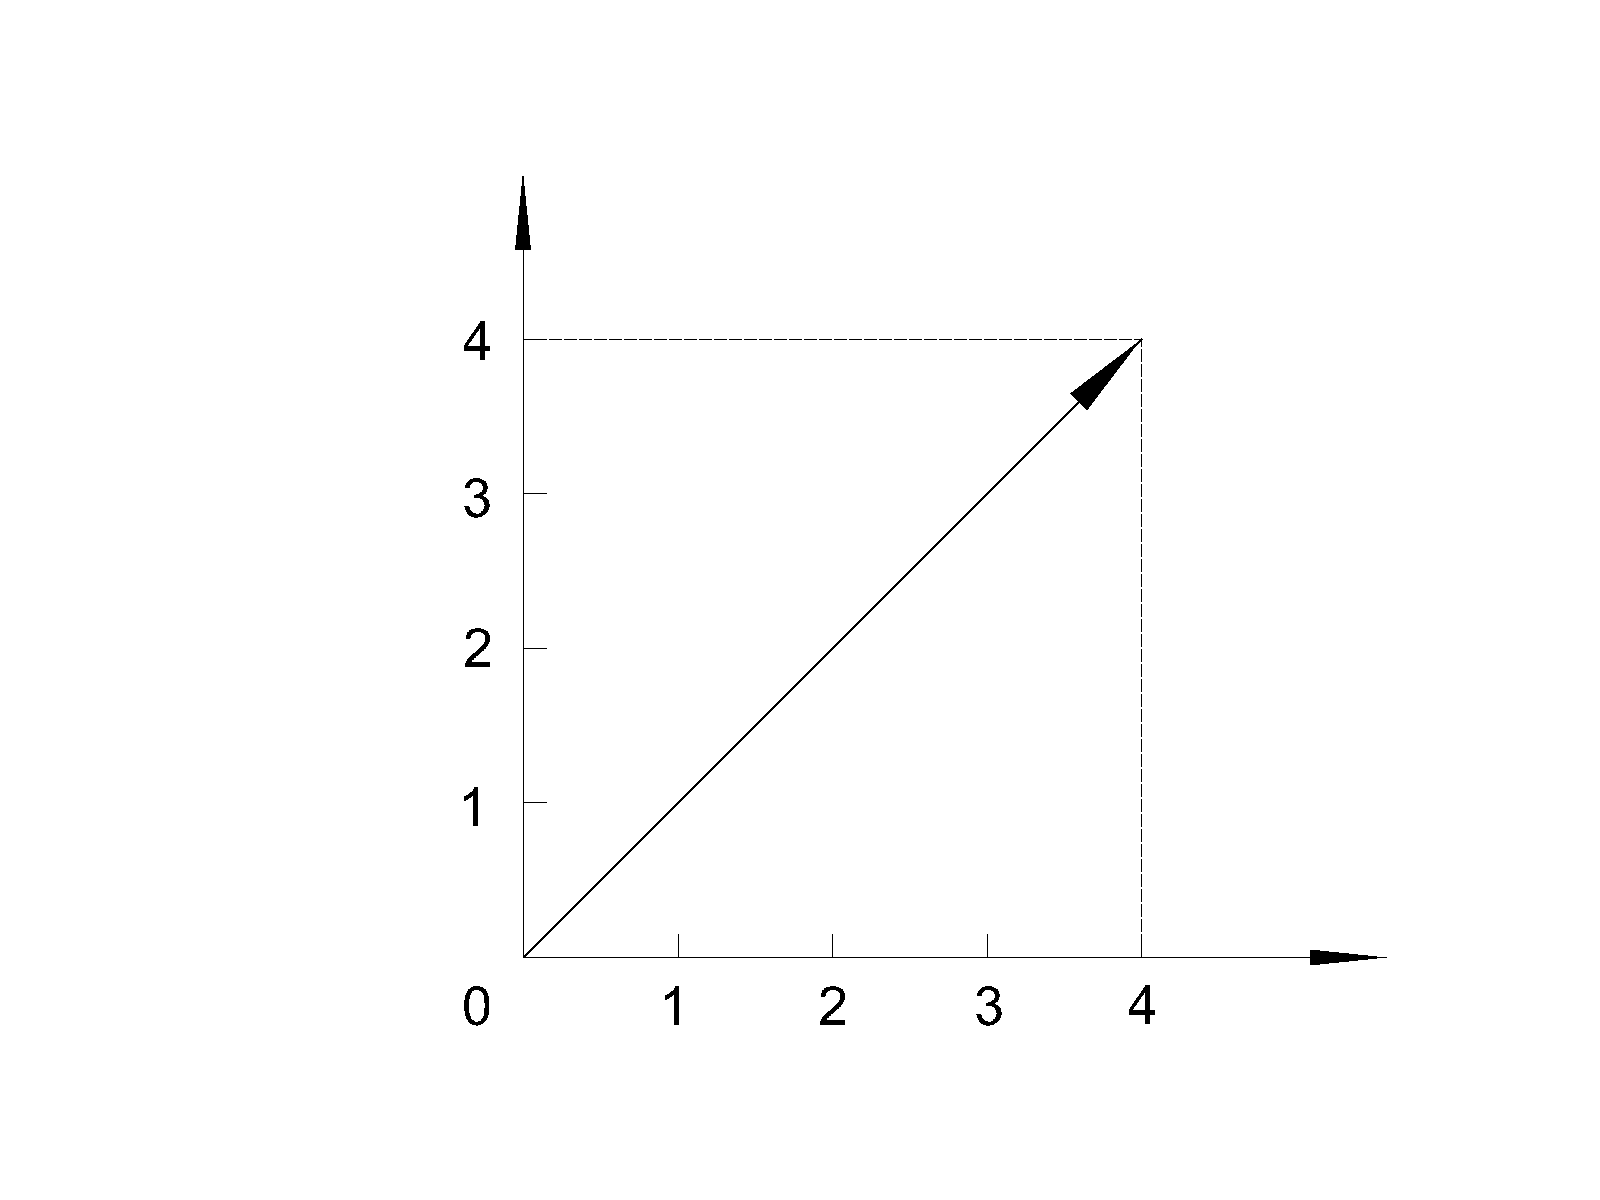
\includegraphics[width=0.60\textwidth]{md230217001}
        \caption{$v_{11}=v_{12}$}
        \label{md230217001}
    \end{figure}
       

    如图\ref{md230217001}所示,此时在该条直线$\left(v_{11}=v_{12}\right)$上任一点所取的值都可作为矩阵的特征向量

    
    取
    $
    \begin{cases}
        v_{11}=1 \\
        v_{12}=1 \\
    \end{cases},
    v_1=
    \left[
        \begin{matrix}
            1 \\ 1 \\
        \end{matrix}
    \right]
    $

    \textcircled{2}当$\lambda=-3$时,带入$(A-\lambda I=0)$,求解矩阵$A$的特征向量

    $$
    \left[
        \begin{matrix}
            1-(-3) & 1 \\
            4 & -2-(-3) \\
        \end{matrix}
    \right]
    \left[
        \begin{matrix}
            v_{21} \\ v_{22} \\
        \end{matrix}
    \right]=0
    \Rightarrow
    4v_{21}+v_{22}=0
    $$

    可取
    $
    \begin{cases}
        v_{21}=1 \\
        v_{22}=-4 \\
    \end{cases},
    v_2=
    \left[
        \begin{matrix}
            1 \\ -4 \\
        \end{matrix}
    \right]
    $

    综上$A$的特征值为$\lambda_1,\lambda_2$,特征向量为
    $
    v_1=
    \left[
        \begin{matrix}
            1 \\ 1 \\
        \end{matrix}
    \right],
    v_2=
    \left[
        \begin{matrix}
            1 \\ -4 \\
        \end{matrix}
    \right]
    $

\end{example}


%-----------------------------------------------------------------------------
%小节
\section{特征值特征向量的应用}

利用特征值特征向量可以对复杂的方程进行画对角,解耦

设$P=\left[v_1,v_2\right]$,$v_1,v_2$是$P$的特征向量,$P$是一个过渡矩阵

\begin{align}
    AP
    &=A
    \left[
        \begin{matrix}
            v_1 & v_2 \\
        \end{matrix}
    \right] 
    \nonumber
    \\
    &=A
    \left[
        \begin{matrix}
            v_{11} & v_{21} \\
            v_{12} & v_{22} \\
        \end{matrix}
    \right] 
    \nonumber
    \\
    &=
    \left[
        \begin{matrix}
            A
            \left[
                \begin{matrix}
                    v_{11} \\ v_{12} \\
                \end{matrix}
            \right] &
            A
            \left[
                \begin{matrix}
                    v_{21} \\ v_{22} \\
                \end{matrix}
            \right] \\
        \end{matrix}
    \right]
    \nonumber
\end{align}

此处由特征值,特征向量的定义可知$Av_1=\lambda_1 v_1,Av_2=\lambda_2 v_2$

\begin{align}
    \mbox{接上式}
    &=
    \left[
        \begin{matrix}
            \lambda_1
            \left[
                \begin{matrix}
                    v_{11} \\ v_{12} \\
                \end{matrix}
            \right] &
            \lambda_2
            \left[
                \begin{matrix}
                    v_{21} \\ v_{22} \\
                \end{matrix}
            \right] \\
        \end{matrix}
    \right]
    \nonumber
    \\
    &=
    \left[
        \begin{matrix}
            \lambda_1v_{11} & \lambda_1v_{12} \\
            \lambda_2v_{21} & \lambda_2v_{22} \\
        \end{matrix}
    \right]
    \nonumber
    \\
    &=
    \left[
        \begin{matrix}
            v_{11} & v_{21} \\
            v_{12} & v_{22} \\
        \end{matrix}
    \right]
    \left[
        \begin{matrix}
            \lambda_1 & 0 \\
            0 & \lambda_2 \\
        \end{matrix}
    \right]
    \nonumber
    \\
    \mbox{令}\Lambda=
    \left[
        \begin{matrix}
            \lambda_1 & 0 \\
            0 & \lambda_2 \\
        \end{matrix}
    \right]
    \nonumber
    \\
    \mbox{可得:}
    \nonumber
    \\
    AP&=P\Lambda
    \nonumber
    \\
    P^{-1}AP&=P^{-1}P\Lambda
    \nonumber
    \\
    P^{-1}AP&=\Lambda
    \nonumber
\end{align}


\begin{example}
    现有微分方程组
    $
    \begin{cases}
        % \mathrm导数d
        \frac{\mathrm{d}x_1}{\mathrm{d}t}=x_1+x_2 \\
        \frac{\mathrm{d}x_2}{\mathrm{d}t}=4x_1-2x_2 \\
    \end{cases}
    $

    解:


    \begin{align}
        \mbox{原式}
        \Rightarrow
        \frac{\mathrm{d}}{\mathrm{d}t}
        \left[
            \begin{matrix}
                x_1 \\
                x_2 \\
            \end{matrix}
        \right]
        &=
        \left[
            \begin{matrix}
                1 & 1 \\
                4 & -2 \\
            \end{matrix}
        \right]
        \left[
            \begin{matrix}
                x_1 \\ x_2 \\
            \end{matrix}
        \right]
        \nonumber
        \\
        \dot x &=Ax
        \label{eq2}
        \\
        \mbox{令}x&=Py
        \nonumber
        \\
        \mbox{可得}
        \Rightarrow
        \begin{cases}
            \dot x=P\dot y \\
            Ax=APy \\
        \end{cases}
        \nonumber
        \\
        \mbox{将上式带回式\ref{eq2}可得:}
        \nonumber
        \\
        P\dot y&=APy
        \nonumber
        \\
        P^{-1}P\dot y&=P^{-1}APy
        \nonumber
        \\
        \dot y&=P^{-1}APy
        \nonumber
        \\
        \mbox{由$P^{-1}AP=\Lambda$可知}
        \nonumber
        \\
        \dot y&=\Lambda y
        \Rightarrow
        \begin{matrix}        
            \dot {y_1} =2y_1 \\
            \dot {y_2} =-3y_2 \\
        \end{matrix}
        \Rightarrow
        \begin{matrix}
            y_1=C_1e^{2t} \\
            y_2=C_2e^{-3t} \\
        \end{matrix}
        \nonumber
        \\
        \mbox{$C_1,C_2$为常数}
        \nonumber
        x&=Py
        \nonumber
        \\
        &=
        \left[
            \begin{matrix}
                1 & 1 \\
                1 & -4 \\
            \end{matrix}
        \right]
        \left[
            \begin{matrix}
                C_1e^{2t} \\
                C_2e^{-3t} \\
            \end{matrix}
        \right]
        \nonumber
        \\
        &=
        \left[
            \begin{matrix}
                C_1e^{2t}+C_2e^{-3t} \\
                C2_e^{2t}-4C_2e^{-3t} \\
            \end{matrix}
        \right]
        \nonumber
        \Lambda=
        \left[
            \begin{matrix}
                \lambda_1 & 0 \\
                0 & \lambda_2 \\
            \end{matrix}
        \right]
        =
        \left[
            \begin{matrix}
                2 & 0 \\
                0 & -3 \\
            \end{matrix}
        \right]
    \end{align}

\end{example}

------------------------------------------------------------------------------
% 小节
\section{总结}

\textcircled{1} $Av=\lambda v$在一条直线上的概念

\textcircled{2} 求解方法 
$
\begin{vmatrix}
    % vmatrix行列式
    A-\lambda I  \\
\end{vmatrix}=0,
(A-\lambda I)V=0
$

\textcircled{3} $P^{-1}AP=\Lambda,P=\left[v_1,v_2...\right],\Lambda=
\left[
    \begin{matrix}
        \lambda_1 && \\
        & \ddots & \\
        && \lambda_n \\
    \end{matrix}
\right]
$

\textcircled{4} $\dot x =Ax,x=Py \dot y=\Lambda y$ 反求$x$



\end{document}
